\section{数学概念}

\subsection{适当函数}
\begin{definition}
    给定函数$f(\cdot)$和非空集合$\mathcal{X}$,如果存在$x\in \mathcal{X}$使得$f(x)< +\infty$,并且对$\forall x in \mathcal{X}$,都有$f(x) > -\infty$,那么称函数$f(\cdot)$关于集合$\mathcal{X}$是适当的
\end{definition}

由定义可知,适当函数$f(\cdot)$具有在某个非空集合$\mathcal{X}$上至少有一处取值不为正无穷,并且处处不为负无穷的特点。

此外,规定适当函数$f(\cdot)$的定义域为$\mathop{\mathrm{dom}} (f) = \{x | f(x) < +\infty\}$.

\subsection{凸函数}
首先引入凸集的概念,直观来看凸集就是任取集合中的两点,其构成的线段都在集合内就称为凸集,下面给出具体的定义。

\begin{definition}
    给定集合$C$,对$\forall x_{1}, x_{2}\in C$,如果对$0 \leq \theta \leq 1$,都有$\theta x_{1}+(1-\theta)x_{2}\in C$,则称这样的集合$C$为凸集
\end{definition}

例如,超平面$\{\bm{x}|\bm{a^{T}}\bm{x}=\bm{b}\}$是典型的凸集,其中$\bm{a}$为任意的非零向量。

\begin{problem}
    超平面$H=\{\bm{x}|\bm{a^{T}}\bm{x}=\bm{b}\}$是凸集。
\end{problem}
\begin{proof}
    任取$\bm{x_{1}}, \bm{x_{2}}\in H, 0 \leq \theta \leq 1$,有
    
    \begin{equation*}
        \begin{cases}
            \bm{a^{T}x_{1}} = \bm{b}, \\
            \bm{a^{T}x_{2}} = \bm{b}.
        \end{cases}
    \end{equation*}

    由$0\leq \theta \leq 1$,进一步可得,
    
    \begin{equation*}
        \begin{cases}
            \theta \bm{a^{T}x_{1}} = \theta \bm{b}, \\
            (1-\theta) \bm{a^{T}x_{2}} = (1-\theta) \bm{b}.
        \end{cases}
    \end{equation*}

    将上述两式相加可得,
    \begin{equation*}
        \begin{split}
            \theta \bm{a^{T}x_{1}} + (1-\theta) \bm{a^{T}x_{2}} &= \theta \bm{b} + (1-\theta) \bm{b} \\
            \bm{a^{T}} (\theta \bm{x_{1}}+(1-\theta)\bm{x_{2}}) &= \bm{b}
        \end{split}
    \end{equation*}

    因此,$\theta \bm{x_{1}}+(1-\theta)\bm{x_{2}} \in H$,即超平面$H$是凸集。
\end{proof}

有了凸集的概念,下面给出凸函数的定义。

\begin{definition}
    设函数$f(\cdot)$是适当函数,如果$\mathop{\mathrm{dom}} (f)$是凸集,且对$\forall x, y\in \mathop{\mathrm{dom}} (f), 0\leq \theta \leq 1$,都有
    \begin{equation}
        f(\theta x+(1-\theta)y) \leq \theta f(x) + (1-\theta)f(y),
    \end{equation}
    则称这样的$f(\cdot)$为凸函数;如果同时还满足$\forall x, y\in \mathop{\mathrm{dom}} (f), x \neq y, 0<\theta<1$,则称这样的$f(\cdot)$为严格凸函数。
\end{definition}

直观来看,连接凸函数图像上的任意两点,其构成的线段都在图像上方。如果连接凸向上的任意两点,其构成的线段都在图像下方,则这样的函数称为凹函数。

例如,负熵函数$f(x)=x\ln x, x>0$是凸函数,其函数图像如\ref{figure_xlnx}所示。

\begin{figure}[hbtp]
    \centering
    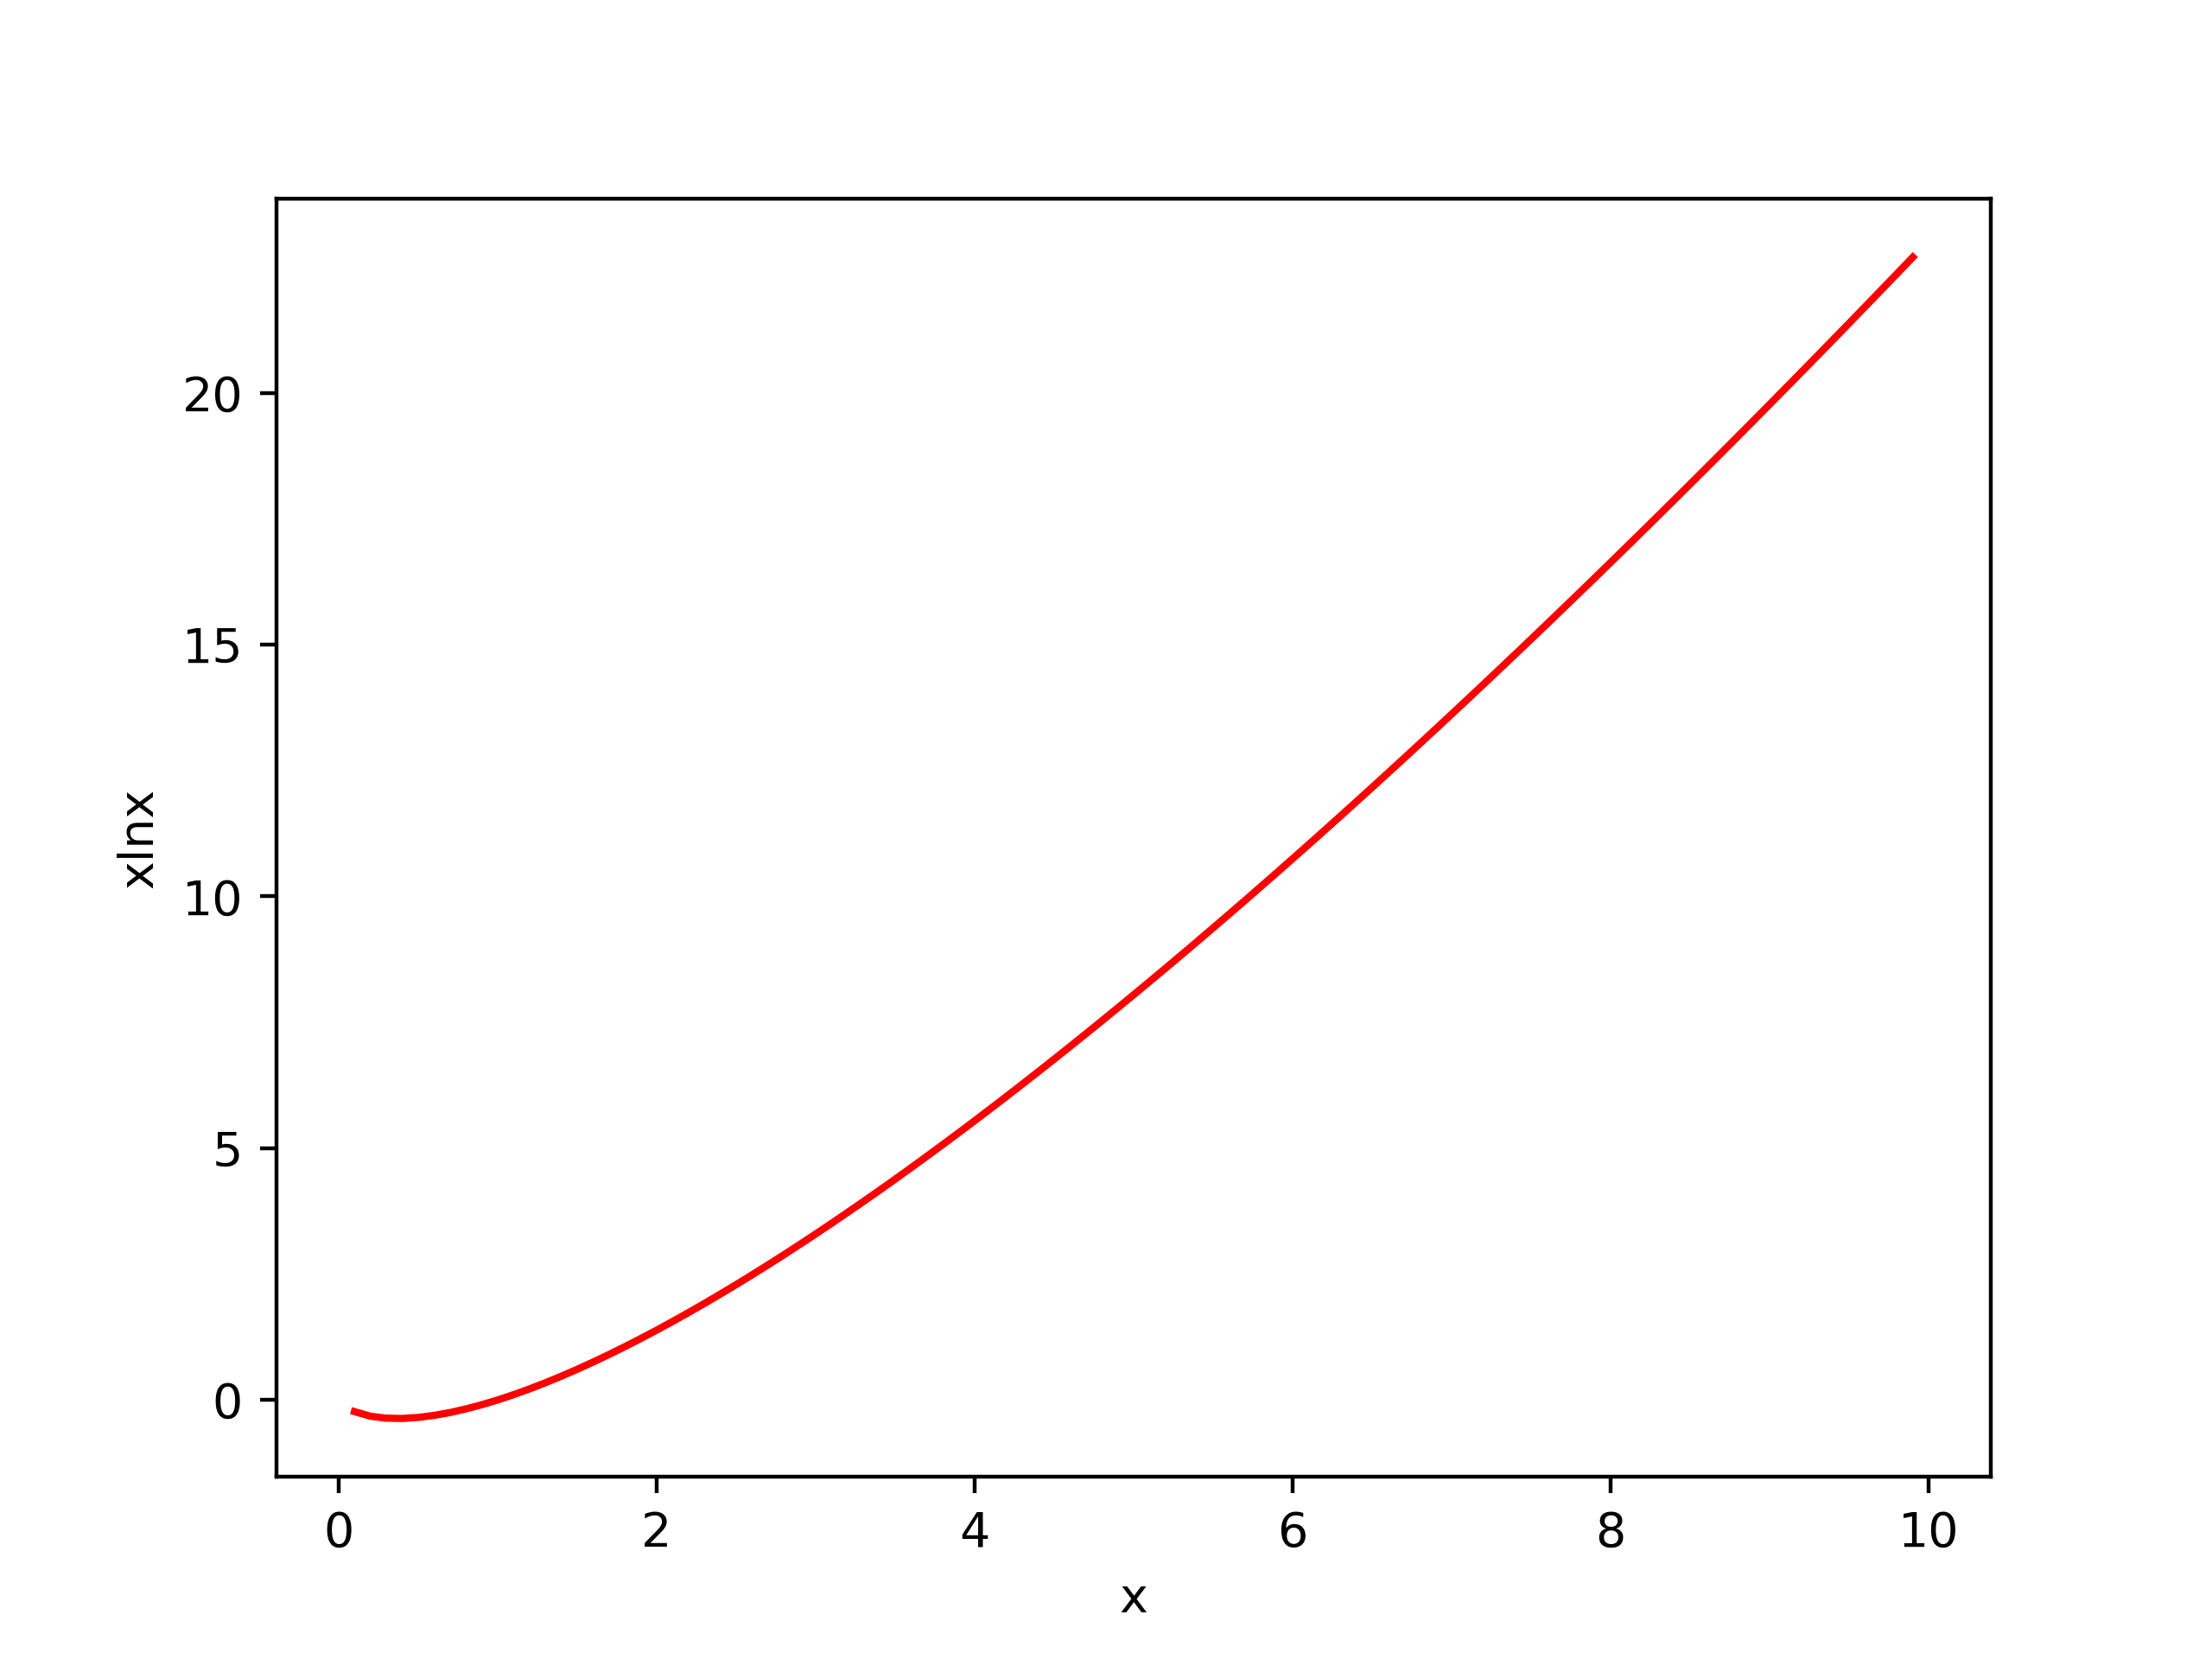
\includegraphics[width=100mm]{./Figures/xlnx_figure.png}
    \caption{$f(x)=x\ln x$函数图像}
    \label{figure_xlnx}
\end{figure}

更进一步,可以定义强凸函数的概念。

\begin{definition}\label{def_convex_1}
    若存在常数$m>0$,使得
    \begin{equation}
        g(x) = f(x) - \frac{m}{2}\|x\|_{2}^{2}
    \end{equation}
    为凸函数,则称这样的$f(\cdot)$为强凸函数或$m$-强凸函数,$m$称为强凸参数。
\end{definition}

由上述的定义,$g(x)$是一个凸函数,因此$g(x)$根据凸函数的定义可以得到如下的等价定义。

\begin{definition}\label{def_convex_2}
    若存在常数$m>0$,使得对$\forall x, y \in \mathop{\mathrm{dom}} (f), 0<\theta<1$,有
    \begin{equation}
        f(\theta x+(1-\theta y)) \leq \theta f(x) + (1-\theta)f(y) - \frac{m}{2}\theta(1-\theta)\|x-y\|_{2}^{2}
    \end{equation}
    则称这样的$f(\cdot)$为强凸函数或$m$-强凸函数,$m$称为强凸参数。
\end{definition}

下面给出上述两个定义是等价的证明。
\begin{proof}
    由定义\ref{def_convex_1}可知,$g(x)$为凸函数,于是有任意的$x, y\in \mathbb{R}, 0<\theta<1$,

    \begin{equation*}
        \begin{split}
            g(\theta x + (1-\theta)y) &\leq \theta g(x) + (1-\theta) g(y) \\
            f(\theta x + (1-\theta)y) - \frac{m}{2}\|\theta x+(1-\theta)y\|_{2}^{2} &\leq \theta(f(x)-\frac{m}{2}\|x\|_{2}^{2}) + (1-\theta) (f(y)-\frac{m}{2}\|y\|_{2}^{2}) \\
            f(\theta x + (1-\theta)y) &\leq \theta f(x) + (1-\theta) f(y) + \frac{m}{2}\theta \|x\|_{2}^{2} - frac{m}{2}(1-\theta)\|y\|_{2}^{2} + \frac{m}{2}\|\theta x + (1-\theta)y\|_{2}^{2} \\
            f(\theta x + (1-\theta)y) &\leq \theta f(x) + (1-\theta) f(y) + \frac{m}{2}\theta(1-\theta)\|x-y\|_{2}^{2}
        \end{split}
    \end{equation*}

    与定义\ref{def_convex_2}的形式相同,因此定义\ref{def_convex_1}和定义\ref{def_convex_2}等价。
\end{proof}

显然,当强凸函数的强凸参数$m=0$时,有$g(x)=f(x)$,即$f(x)$退化成了一个凸函数。此外,根据等价定义,也可以得到$f(x)$同时是一个严格凸函数。因此,强凸函数一定是严格凸函数,当$m=0$时退化成凸函数。

下面考虑强凸函数关于最小值的定理。

\begin{theorem}
    设$f(\cdot)$是强凸函数,且$f(\cdot)$存在最小值,则最小值点唯一。
\end{theorem}
\begin{proof}
    假设$f(\cdot)$存在两个不同的点$x\neq y, x, y\in \mathop{\mathrm{dom}} (f)$都是$f(\cdot)$的最小值点,

    那么由强凸函数的等价定义,对$\forall 0<\theta<1, m>0$,有
    \begin{equation*}
        \begin{split}
            f(\theta x + (1-\theta)y) &\leq \theta f(x) + (1-\theta)f(y) - \frac{m}{2}\theta(1-\theta)\|x-y\|_{2}^{2} \\
            &= f(x) - \frac{m}{2}\theta(1-\theta)\|x-y\|_{2}^{2} \\
            &< f(x)
        \end{split}
    \end{equation*}
    与假设$f(x)$为最小值矛盾,因此假设不成立,即如果$f(\cdot)$是强凸函数,且$f(\cdot)$存在最小值,则最小值点唯一。
\end{proof}

最后分析凸函数的一些基本性质。
\begin{theorem}
    若$f_{1}, f_{2}$是凸函数,则$f_{1}+f_{2}$也是凸函数
\end{theorem}
\begin{proof}
    由$f_{1}, f_{2}$是凸函数可知,对$\forall x, y\in \mathop{\mathrm{dom}} (f), 0\leq \theta \leq 1$有

    \begin{equation*}
        \begin{split}
            f_{1}(\theta x+(1-\theta)y)+f_{2}(\theta x+(1-\theta)y) &\leq \theta f_{1}(x)+(1-\theta)f_{1}(y) + \theta f_{2}(x)+(1-\theta)f_{2}(y) \\
            &=\theta(f_{1}(x)+f_{2}(x)) + (1-\theta)(f_{1}(y)+f_{2}(y))
        \end{split}
    \end{equation*}
    由凸函数的定义,$f_{1}+f_{2}$是凸函数。
\end{proof}

\begin{theorem}
    若$f_{1}, f_{2}, \cdots, f_{m}$是凸函数,则$f(x)=\mathop{\mathrm{max}}\{ f_{1}, f_{2}, \cdots, f_{m}\}$也是凸函数
\end{theorem}
\begin{proof}
    对$\forall x, y\in \mathop{\mathrm{dom}} (f), 0\leq \theta \leq 1$,有
    
    \begin{equation*}
        \begin{split}
            f(\theta x + (1-\theta) y) &=\mathop{\mathrm{max}} \{f_{1}(\theta x + (1-\theta) y), f_{2}(\theta x + (1-\theta) y), \cdots, f_{m}(\theta x + (1-\theta) y)\} \\
            &\leq \mathop{\mathrm{max}} \{\theta f_{1}(x) + (1-\theta)f_{1}(y), \theta f_{2}(x) + (1-\theta)f_{2}(y), \cdots, \theta f_{m}(x) + (1-\theta)f_{m}(y)\} \\
        \end{split}
    \end{equation*}

    注意到$f(x) = \mathop{\mathrm{max}} \{f_{1}, f_{2}, \cdots, f_{m}\}$,因此$f(x)\leq f_{i}(x), i=1,2,\cdots,m$,于是可以得到,

    \begin{equation*}
        f(\theta x + (1-\theta) y) \leq \theta f(x) + (1-\theta)f(y)
    \end{equation*}
    由凸函数的定义,$f(x)=\mathop{\mathrm{max}}\{ f_{1}, f_{2}, \cdots, f_{m}\}$是凸函数。
\end{proof}

\begin{definition}[聚点]
    任给$\varepsilon>0$,存在无穷多个$z_{n}$满足
    \begin{equation}
        \left|z_{n}-z\right|<\varepsilon .
        \nonumber
    \end{equation}
    则称$z$为复数序列$\left\{z_{n}\right\}$的一个聚点。
\end{definition}


% \subsection{范数}

% 在欧氏空间中,对于距离的定义是一个宽泛的概念,只要满足非负、自反、三角不等式就可以称之为距离。
% 而范数是一种强化了的距离概念,它在定义上比距离多了一条数乘的运算法则。
% \begin{theorem}[非负性]
%     对于任意的$x\in \mathbb{R}^{n}$,有$\|x\|\geq0$,其中$\|x\|=0$当且仅当$x=0$
% \end{theorem}
% \begin{theorem}[齐次性]
%     对于任意的$x\in \mathbb{R}^{n}$和$\lambda \in R $,有$\|\lambda x\| = |\lambda|\|x\|$
% \end{theorem}
% \begin{theorem}[三角不等式]
%     对于任意的$x\in \mathbb{R}^{n}$和$y \in \mathbb{R}^{n} $,有$\|x+y\| \leq  \|x\| + \|y\|$
% \end{theorem}

% 在数学上,范数包括向量范数和矩阵范数,向量范数表征向量空间中向量的大小,矩阵范数表征矩阵引起变化的大小。
% 以下介绍几种向量范数的定义和含义 

% \subsubsection{$l_0$范数}
% $l_0$范数并不是一个真正的范数,它主要被用来度量向量中非零元素的个数。
% L-0的定义为: 
% \begin{equation}
%     \|x\|_0: = \sqrt[0]{\sum_{i=1}^nx_i^0}
% \end{equation}
% 为了避免0的0次方,以及非零数开0次方等问题,使用的格式是: 
% \begin{equation}
%     \|x\|_0 := \neq (i|x_i\neq0)
% \end{equation}

% 表示向量x中非零元素的个数。对于$l_0$范数,其优化问题为: 
% \begin{equation}
%     \mathrm{min}\|x\|_0  \quad\quad \mathrm{s. t.}Ax=b
% \end{equation}

% 在实际应用中,由于$l_0$范数本身不容易有一个好的数学表示形式。所以在实际情况中,$l_0$的最优问题会被放宽到$l_1$或$l_2$下的最优化。

% \subsubsection{$l_1$范数}
% $l_1$范数是常用的一种范数,它的定义如下:
% \begin{equation}
%     \|x\|_1=\sum_{i=1}^n|x_i|
% \end{equation}
% 表示向量x中非零元素的绝对值之和。$l_1$范数也被称作曼哈顿距离、最小绝对误差等。
% 使用$l_1$范数可以度量两个向量间的差异,如绝对误差和(Sum of Absolute Difference):
% \begin{equation}
%     \mathrm{SAD}(x_1,x_2) = \sum_i^n|x_{1i}-x_{2i}|
% \end{equation}
% 对于$l_1$范数,它的优化问题如下:
% \begin{equation}
%     \mathrm{min}\|x\|_1 \quad\quad \mathrm{s. t.} Ax = b
% \end{equation}

% 由于$l_1$范数的天然性质,对$l_1$优化的解是一个稀疏解,因此$l_1$范数也被叫做稀疏规则算子。通过$l_1$可以实现特征的稀疏,去掉一些没有信息的特征。

% \subsubsection{$l_2$范数}
% $l_2$范数是最常见最常用的范数,我们用的最多的度量距离欧氏距离就是一种$l_2$范数,它的定义如下:
% \begin{equation}
%     \|x\|_2 = \sqrt{\sum_{i=1}^nx_i^2}
% \end{equation}
% 表示向量元素的平方和再开平方。 像$l_1$范数一样,$l_2$也可以度量两个向量间的差异,如平方差和(Sum of Squared Difference):
% \begin{equation}
%     \mathrm{SSD}(x_1,x_2) = \sum_{i=1}^n(x_{1i}-x_{2i})^2
% \end{equation}
% 对于$l_2$范数,它的优化问题如下:
% \begin{equation}
%     \mathrm{min}\|x\|_2 \quad\quad \mathrm{s. t.}Ax = b
% \end{equation}

% $l_2$范数通常会被用来做优化目标函数的正则化项,防止模型为了迎合训练集而过于复杂造成过拟合的情况,从而提高模型的泛化能力。

% \subsubsection{无穷范数}
% 对于无穷范数,存在着与先前范数类似的定义:
% \begin{equation}
%     \|x\|_\infty = \sqrt[\infty]{\sum_{i=1}^nx_i^{\infty}}
% \end{equation}
% 它主要被用来度量向量元素的最大值,与$l_0$一样,通常情况下表示为:
% \begin{equation}
%     \|x\|_{\infty} := max\{|x_1|,|x_2|,...,|x_n|\}.
% \end{equation}

\begin{definition}[向量内积]
    给定向量$\bm{x} \in \mathbb{R}^{n}$和$\bm{y} \in \mathbb{R}^{n}$, 定义两个向量的内积为
    \begin{equation}
        \langle\bm{x}, \bm{y}\rangle=\sum_{i=1}^{n} x_{i} y_{i},
        \nonumber
    \end{equation}
如果$\langle\bm{x}, \bm{y}\rangle=0$, 则记为$\bm{x} \perp \bm{y}$。
\end{definition}

\begin{theorem}[柯西-施瓦茨不等式]
    对任意的$  \bm{x} \in \mathbb{R}^{n}  $和$  \bm{y} \in \mathbb{R}^{n}  $有
    \begin{equation}
    |\langle\bm{x}, \bm{y}\rangle| \leq\|\bm{x}\| \cdot\|\bm{y}\|,
        \nonumber
    \end{equation}
    该不等式称为柯西-施瓦茨不等式(Cauchy-Schwarz inequality)\cite{2007柯西}。
    \label{thm1_4}
\end{theorem}
\begin{proof}
    设$x=(x_1,x_2...x_n),y=(y_1,y_2...y_n)$,则
    \begin{equation}
        |\langle\bm{x}, \bm{y}\rangle|^2=(\bm{x}_1\bm{y}_1+...+\bm{x}_n\bm{y}_n)^2, \\
        \|\bm{x}\|^2 \cdot\|\bm{y}\|^2=(\bm{x}_1^2+...+\bm{x}_n^2) \cdot(\bm{y}_1^2+...+\bm{y}_n^2), \\
        \nonumber
    \end{equation}
    构造方程
    \begin{equation}
        (\bm{x}_1\bm{z}-\bm{y}_1)^2+...+(\bm{x}_n\bm{z}-\bm{y}_n)^2=0,
        \nonumber
    \end{equation}
    其中$\bm{z} \in \mathbb{R}^{n}$且为未知数。将方程拆分成以下形式
    \begin{equation}
        (\bm{x}_1^2+...+\bm{x}_n^2)\bm{z}^2-2(\bm{x}_1\bm{y}_1+...+\bm{x}_n\bm{y}_n)\bm{z}+(\bm{y}_1^2+...+\bm{y}_n^2)=0,
        \nonumber
    \end{equation}
    因为方程参数固定,只有一个未知数,因此至多只有一个解,即$\Delta \leq 0$,也即
    \begin{equation}
        \Delta=4(\bm{x}_1\bm{y}_1+...+\bm{x}_n\bm{y}_n)^2-4(\bm{x}_1^2+...+\bm{x}_n^2)(\bm{y}_1^2+...+\bm{y}_n^2) \leq 0 ,
        \nonumber
    \end{equation}
    故
    \begin{equation}
        |\langle\bm{x}, \bm{y}\rangle| \leq\|\bm{x}\| \cdot\|\bm{y}\|.
        \nonumber
    \end{equation}
    不等式成立。
\end{proof}

\subsection{梯度与次梯度}
\begin{definition}[梯度]
    给定函数 $f: \mathbb{R}^{n} \rightarrow \mathbb{R}$ 在 $\bm{x} \in \mathbb{R}^{n}$ 的梯度定义为:
\begin{equation}
    \nabla f(\bm{x}):=\left(\begin{array}{c}
    \frac{\partial f(\bm{x})}{\partial x_{1}} \\
    \vdots \\
    \frac{\partial f(x)}{\partial x_{n}}
    \end{array}\right),
    \nonumber
\end{equation}
其中 $\frac{\partial f(x)}{\partial x_{i}}:=\lim _{t \rightarrow 0} \frac{f\left(x+t e_{i}\right)-f(x)}{t}$ , $e_{i}$ 为第 $\bm{i}$ 个元素为 1 的单位向量 $(0, \cdots, 1, \cdots, 0)^{\top}$ 。 
\end{definition}

\begin{definition}[次梯度]
    函数$f: \mathbb{R}^{n} \rightarrow \mathbb{R}$是一个适当的函数且对于$\bm{x} \in \operatorname{dom}(f)$, 如果向量$\bm{g} \in \mathbb{R}^{n}$满足
    \begin{equation}
        f(\bm{y}) \geq f(\bm{x})+\langle\bm{g}, \bm{y}-\bm{x}\rangle, \forall \bm{y} \in \mathbb{R}^{n}, \bm{y} \in \operatorname{dom}(f) ,
        \nonumber
    \end{equation}
    则称$\bm{g}$为函数$f(\cdot)$在$\bm{x}$处的一个次梯度 (sub-gradient)。
\end{definition}

\begin{definition}[次微分]
    函数$f: \mathbb{R}^{n} \rightarrow \mathbb{R}$在$\bm{x} \in \operatorname{dom}(f)$的所有次梯度的集合称为函数$f(\cdot)$在$\bm{x}$的次微分 (sub-differential),记为$\partial f(\bm{x})$:
    \begin{equation}
        \partial f(\bm{x}):=\left\{\bm{g} \in \mathbb{R}^{n} \mid f(\bm{y}) \geq f(\bm{x})+\langle\bm{g}, \bm{y}-\bm{x}\rangle, \forall \bm{y} \in \operatorname{dom}(f)\right\} .
        \nonumber
    \end{equation}
\end{definition}



\subsection{海塞矩阵}
海塞矩阵(Hesse矩阵),是一个多元函数的二阶偏导数构成的方阵,常用于牛顿法解决优化问题:
若一元函数$f(x)$在$x=x_0$点的某个邻域内具有任意阶导数,则$f(x)$在$x_0$点处的泰勒展开式为:
\begin{equation}
    f(x) = f(x_0) + f'(x_0)\Delta x + \frac{1}{2}f''(x_0)(\Delta x)^2 + ...
\end{equation}

其中 $\Delta x = x - x_0$, $\Delta x^2 = (x - x_0)^2$

二元函数$f(x_1,x_2)$在$X_0(x_0,y_0)$点处的泰勒展开式为:
\begin{equation}
    f(x,y) = f(x_0,y_0)
        + \left.\displaystyle\frac{\partial f}{\partial x}\right|_{X_0}\Delta x_0    
        + \left.\displaystyle\frac{\partial f}{\partial y}\right|_{X_0}\Delta y_0    
        + \frac{1}{2}
        \left[ \left.\displaystyle\frac{\partial^2f}{\partial x^2}\right|_{X_0}\Delta x_0^2 + 
          2\left.\displaystyle\frac{\partial^2f}{\partial x\partial y}\right|_{X_0}\Delta x_0\Delta y_0 + 
          \left.\displaystyle\frac{\partial^2f}{\partial y^2}\right|_{X_0}\Delta y_0^2 \right]   
        + ...
\end{equation}

其中$\Delta x = x - x_0$,$\Delta y = y - y_0$.
将上述展开式写成矩阵形式,则有:

\begin{equation}
    f(X) = f(X_0) 
    + \left.( \displaystyle\frac{\partial f}{\partial x},
        \displaystyle\frac{\partial f}{\partial y} )\right|_{X_0}    
        \begin{pmatrix}
             \Delta x \\
             \Delta y
        \end{pmatrix}
    +\newline \frac{1}{2}(\Delta x, \Delta y)
        \left.
        \begin{pmatrix}
            \displaystyle\frac{\partial^2f}{\partial x^2} & \displaystyle\frac{\partial^2f}{\partial x\partial y} \\
            \displaystyle\frac{\partial^2f}{\partial y\partial x} & \displaystyle\frac{\partial^2f}{\partial y^2}
        \end{pmatrix}
        \right|_{X_0}
        \begin{pmatrix}
             \Delta x \\
             \Delta y
        \end{pmatrix}
\end{equation}

即:
\begin{equation}
    f(X) = f(X_0) + \nabla f(X_0)^{\mathbb{T}}\Delta X + \frac{1}{2}X^{\mathbb{T}}G(X_0)\Delta X + ...\quad.
\end{equation}
其中:
\begin{equation}
    G(X_0) = 
        \left.
        \begin{pmatrix}
            \displaystyle\frac{\partial^2f}{\partial x^2} & \displaystyle\frac{\partial^2f}{\partial x\partial y} \\
            \displaystyle\frac{\partial^2f}{\partial y\partial x} & \displaystyle\frac{\partial^2f}{\partial y^2}
        \end{pmatrix}
        \right|_{X_0},
    \Delta X = 
        \begin{pmatrix}
             \Delta x \\
             \Delta y
        \end{pmatrix}.
\end{equation}


  $G(X_0)$是$f(x,y)$在$X_0$点处的Hesse矩阵。它是由函$f(x,y)$在$X_0$点处的二阶偏导数所组成的方阵。
将二元函数的泰勒展开式推广到多元函数,则$f(x_1,x_2...,x_n)$在$X_0$点处的泰勒展开式的矩阵形式为:
\begin{equation}
    f(X) = f(X_0) + \nabla f(X_0)^T\Delta X + \frac{1}{2}X^TG(X_0)\Delta X + ...\quad.
\end{equation}
其中:

(1)$\nabla f(X_0) = \left.\left[ 
        \displaystyle\frac{\partial f}{\partial x_1},
        \displaystyle\frac{\partial f}{\partial x_2},
        ...,
        \displaystyle\frac{\partial f}{\partial x_n} \right]\right|_{X_0}^T$,它是$f(X)$在$X_0$点处的梯度。
        
(2)$ G(X_0) = 
        \left.
        \begin{pmatrix}
            \displaystyle\frac{\partial^2f}{\partial x_1^2} & \displaystyle\frac{\partial^2f}{\partial x_1\partial x_2} & \cdots & \displaystyle\frac{\partial^2f}{\partial x_1\partial x_n}\\
            \displaystyle\frac{\partial^2f}{\partial x_2\partial x_1} & \displaystyle\frac{\partial^2f}{\partial x_2^2} & \cdots & \displaystyle\frac{\partial^2f}{\partial x_2\partial x_n}\\
            \vdots & \vdots & \ddots & \vdots\\
            \displaystyle\frac{\partial^2f}{\partial x_n\partial x_1} & \displaystyle\frac{\partial^2f}{\partial x_n\partial x_2} & \cdots & \displaystyle\frac{\partial^2f}{\partial x_n^2}\\
        \end{pmatrix}
        \right|_{X_0}$
        为$f(X)$在$X_0$点处的Hesse矩阵。
\begin{definition}[Hesse矩阵]
    Hesse矩阵是由目标函数 $f(\cdot)$ 在点 $X$ 处的二阶偏导数组成的 $n\times n$ 阶对称矩阵。       
\end{definition}

% 8
\subsection{李普希茨连续可微与$L-$光滑性质}
\begin{definition}[李普希茨连续]
    如果函数$f: \mathbb{R}^{n} \rightarrow \mathbb{R}$是适当的凸函数,且满足
\begin{equation}
    |f(\bm{x})-f(\bm{y})| \leq L\|\bm{x}-\bm{y}\|, \forall \bm{x}, \bm{y} \in \operatorname{dom}(f),
    \nonumber
\end{equation}
则我们认为函数$f(\cdot)$是李普希茨 (Lipschitz) 连续的,其中常数$L$称为光滑参数。
\end{definition}

\begin{definition}[$L-$光滑]
    给定$L \geq 0$, 函数$f: \mathbb{R}^{n} \rightarrow \mathbb{R}$定义在集合$\mathcal{D}$上是可微的,且满足
\begin{equation}
    \|\nabla f(\bm{x})-\nabla f(\bm{y})\| \leq L\|\bm{x}-\bm{y}\|, \quad \forall \bm{x}, \bm{y} \in \mathcal{D},
    \nonumber
\end{equation}
则该函数$f(\cdot)$是$L-$光滑的,而常数$L$称为光滑参数。
\end{definition}

\begin{problem}[二次函数的$L-$光滑]
    考虑二次函数$f: \mathbb{R}^{n} \rightarrow \mathbb{R}$是
    \begin{equation}
        f(\bm{x})=\frac{1}{2} \bm{x}^{\top} \bm{A} \bm{x}+\bm{b}^{\top} \bm{x}+c,
        \nonumber
    \end{equation}
其中$\bm{A} \in \mathbb{R}^{n}$为对称矩阵且$c \in \mathbb{R}$。证明$\|\bm{A}\|_{p, q}$是最小的光滑参数,其中$\|\cdot\|_{p, q}$表示诱导范数,即
    \begin{equation}
        \|\bm{A}\|_{p, q}=\max \left\{\|\bm{A} \bm{x}\|_{q} \mid\|\bm{x}\|_{p} \leq 1\right\},
        \nonumber
    \end{equation}
要求$q \in[1, \infty)$且$\frac{1}{p}+\frac{1}{q}=1$。
\end{problem}
\begin{solution}
    考虑定义在$\mathbb{R}^{n}$上的一般$l_{p} -$范数$(1 \leq p \leq \infty)$。那么对任意的$\bm{x}, \bm{y} \in \mathbb{R}^{n}$,
    \begin{equation}
        \|\nabla f(\bm{x})-\nabla f(\bm{y})\|_{q}=\|\bm{A} \bm{x}-\bm{A} \bm{y}\|_{q} \leq\|\bm{A}\|_{p, q}\|\bm{x}-\bm{y}\|_{p},
        \nonumber
    \end{equation}
    依题意,
    \begin{equation}
        \|\bm{A}\|_{p, q}=\max \left\{\|\bm{A} \bm{x}\|_{q} \mid\|\bm{x}\|_{p} \leq 1\right\},
        \nonumber
    \end{equation}
    我们可以说明函数$f(\cdot)$是$\|\bm{A}\|_{p, q}$光滑的。特别需要说明的是,$\|\bm{A}\|_{p, q}$是最小的光滑参数。加入函数$f(\cdot)$是$L -$光滑的,那么取一个 $\tilde{\bm{x}}$满足$\|\tilde{\bm{x}}\|_{p}=1$和$ \|\bm{A} \tilde{\bm{x}}\|_{q}=\|\bm{A}\|_{p, q}$,那么
    \begin{equation}
        \|\bm{A}\|_{p, q}=\|\bm{A} \tilde{\bm{x}}\|_{q}=\|\nabla f(\tilde{\bm{x}})-\nabla f(\mathbf{0})\|_{q} \leq L\|\tilde{\bm{x}}-\mathbf{0}\|_{p}=L,
        \nonumber
    \end{equation}
从而说明$\|\bm{A}\|_{p, q}$是最小的光滑参数。
\end{solution}
\par 下面介绍关于 L-光滑函数的非常有用的结论,即下降引理(Descent Lemma),该引理所表达的是该函数有一个特定的二次函数上界。

\begin{theorem}[下降引理]
    如果函数$f: \mathbb{R}^{n}\rightarrow \mathbb{R}$是一个定义在给定凸集$D$上的$L$-光滑函数,那么对于$\forall \bm{x}, \bm{y}\in D$,有
    \begin{equation}
        f(y) \leq f(\bm{x}) + \langle \nabla f(\bm{x}), \bm{y}-\bm{x} \rangle + \frac{L}{2}\|\bm{x}-\bm{y}\|_{2}^{2}
    \end{equation}
    \label{thm435}
\end{theorem}

\begin{proof}
    由微积分基本定理,
    
    \begin{equation*}
        f(\bm{y}) - f(\bm{x}) = \int_{0}^{1}\langle \nabla f(\bm{x} + t(\bm{y} - \bm{x})), \bm{y}-\bm{x}\rangle dt
    \end{equation*}

    因此,

    \begin{equation*}
        f(\bm{y}) - f(\bm{x}) = \langle \nabla f(\bm{x}), \bm{y}-\bm{x}\rangle + \int_{0}^{1}\langle \nabla f(x+t(\bm{y}-\bm{x})) - \nabla f(\bm{x}), \bm{y}-\bm{x}\rangle dt
    \end{equation*}

    进一步可以得到,

    \begin{equation*}
        \begin{split}
            |f(\bm{y}) - f(\bm{x}) - \langle \nabla f(\bm{x}), \bm{y}-\bm{x}\rangle| &= |\int_{0}^{1}\langle \nabla f(x+t(\bm{y}-\bm{x})) - \nabla f(\bm{x}), \bm{y}-\bm{x}\rangle dt| \\
            &\leq \int_{0}^{1} |\langle \nabla f(x+t(\bm{y}-\bm{x})) - \nabla f(\bm{x}), \bm{y}-\bm{x}\rangle| dt
        \end{split}
    \end{equation*}

    由Cauchy-Schwarz不等式可得,
    \begin{equation*}
        \begin{split}
            |f(\bm{y}) - f(\bm{x}) - \langle \nabla f(\bm{x}), \bm{y}-\bm{x}\rangle| &\leq \|\nabla f(x+t(\bm{y}-\bm{x})) - \nabla f(\bm{x})\|_{2} \cdot \|\bm{y}-\bm{x}\|_{2} dt \\
            &\leq \int_{0}^{1} tL\|\bm{y}-\bm{x}\|_{2}^{2}dt \\
            &= \frac{L}{2} \|\bm{y}-\bm{x}\|_{2}^{2}
        \end{split}
    \end{equation*}

    整理可得,
    \begin{equation*}
        f(\bm{y}) \leq f(\bm{x}) + \langle \nabla f(\bm{x}), \bm{y}-\bm{x} \rangle + \frac{L}{2}\|\bm{x}-\bm{y}\|_{2}^{2}
    \end{equation*}
\end{proof}



\begin{theorem}[$L-$光滑的多种刻画性质]
    如果函数$f: \mathbb{R}^{n} \rightarrow \mathbb{R}$是一个连续可微凸函数,那么下面的性质均是等价的:
\par     i). $f(\cdot)$是$L -$光滑的; 
\par    ii). 对任意的$\bm{x}, \bm{y} \in \mathbb{R}^{n}$,
    \begin{equation}
        f(\bm{y}) \leq f(\bm{x})+\langle\nabla f(\bm{x}), \bm{y}-\bm{x}\rangle+\frac{L}{2}\|\bm{x}-\bm{y}\|^{2} .
        \nonumber
    \end{equation} 
\par    iii). 对任意的$\bm{x}, \bm{y} \in \mathbb{R}^{n}$,
    \begin{equation}
        f(\bm{y}) \geq f(\bm{x})+\langle\nabla f(\bm{y}), \bm{y}-\bm{x}\rangle+\frac{1}{2 L}\|\nabla f(\bm{x})-\nabla f(\bm{y})\|^{2} .
        \nonumber
    \end{equation}
\par    iv). 对任意的$\bm{x}, \bm{y} \in \mathbb{R}^{n}$,
    \begin{equation}
        \langle\nabla f(\bm{x})-\nabla f(\bm{y}), \bm{x}-\bm{y}\rangle \geq \frac{1}{L}\|\nabla f(\bm{x})-\nabla f(\bm{y})\|^{2} .
        \nonumber
    \end{equation}
\par     v). 对任意的$\bm{x}, \bm{y} \in \mathbb{R}^{n}$和$\lambda \in[0,1]$,
    \begin{equation}
        f(\lambda \bm{x}+(1-\lambda) \bm{y}) \geq \lambda f(\bm{x})+(1-\lambda) f(\bm{y})-\frac{L}{2} \lambda(1-\lambda)\|\bm{x}-\bm{y}\|^{2} .
        \nonumber
    \end{equation}
    \label{thm1_1}
\end{theorem}
\begin{proof}
    i)$  \Rightarrow  $ii):由下降引理得到;\\
ii)$  \Rightarrow  $iii):假设$  \nabla f(\bm{x})=\nabla f(\bm{y}) $,对于给定的$  \bm{x} \in \mathbb{R}^{n}$,考虑
\begin{equation}
g_{x}(\bm{y})=f(\bm{y})-f(\bm{x})-\langle\nabla f(\bm{x}), \bm{y}-\bm{x}\rangle, \bm{y} \in \mathbb{R}^{n},
    \nonumber
\end{equation}
对于该函数$g_{x}(\cdot)$,有
\begin{equation}
\begin{aligned}
g_{\bm{x}}(\bm{z}) &=f(\bm{z})-f(\bm{x})-\langle\nabla f(\bm{x}), \bm{z}-\bm{x}\rangle \\
& \leq f(\bm{y})+\langle\nabla f(\bm{y}), \bm{z}-\bm{y}\rangle+\frac{L}{2}\|\bm{z}-\bm{y}\|^{2}-f(\bm{x})-\langle\nabla f(\bm{x}), \bm{z}-\bm{x}\rangle \\
&=f(\bm{y})-f(\bm{x})-\langle\nabla f(\bm{x}), \bm{y}-\bm{x}\rangle+\langle\nabla f(\bm{y})-\nabla f(\bm{x}), \bm{z}-\bm{y}\rangle+\frac{L}{2}\|\bm{z}-\bm{y}\|^{2} \\
&=g_{x}(\bm{y})+\left\langle\nabla g_{x}(\bm{y}), \bm{z}-\bm{y}\right\rangle+\frac{L}{2}\|\bm{z}-\bm{y}\|^{2}
\end{aligned}
    \nonumber
\end{equation}
注意到,$\nabla g_{\bm{x}}(\bm{y})=\nabla f(\bm{y})-\nabla f(\bm{x})  $对任意的$  \bm{y} \in \mathbb{R}^{n}  $成立。如果$  \nabla g_{\hat{\bm{x}}}(\cdot)=0 $,结合函数$g_{x}(\cdot)$的凸性,$\hat{\bm{x}}  $是$g_{x}(\cdot)$的全局最小解, 即
\begin{equation}
g_{x}(\hat{\bm{x}}) \leq g_{x}(\bm{z}), \quad \forall \bm{z} \in \mathbb{R}^{n} .
    \nonumber
\end{equation}
另$  \bm{y} \in \mathbb{R}^{n}  $和$  \bm{v} \in \mathbb{R}^{n} $,且$  \|\bm{v}\|=1  $以及$  \left\langle\nabla g_{x}(\bm{y}), \bm{v}\right\rangle=\left\|\nabla g_{x}(\bm{y})\right\|$,将
\begin{equation}
    \bm{z}=\bm{y}-\frac{\left\|\nabla g_{x}(\bm{y})\right\|}{L} \bm{v},
    \nonumber
\end{equation}
代入到
\begin{equation}
0=g_{x}(\bm{x}) \leq g_{x}\left(\bm{y}-\frac{\left\|\nabla g_{x}(\bm{y})\right\|}{L} \bm{v}\right) .
    \nonumber
\end{equation}
进一步根据函数$  g_{x}  $的性质,有
\begin{equation}
\begin{aligned}
0 &=g_{\bm{x}}(\bm{x}) \\
& \leq g_{\bm{x}}(\bm{y})-\frac{\left\|\nabla g_{\bm{x}}(\bm{y})\right\|}{L}\left\langle\nabla g_{x}(\bm{y}), \bm{v}\right\rangle+\frac{1}{2 L}\left\|\nabla g_{\bm{x}}(\bm{y})\right\|^{2} \cdot\|\bm{v}\|^{2} \\
&=g_{\bm{x}}(\bm{y})-\frac{1}{2 L}\left\|\nabla g_{\bm{x}}(\bm{y})\right\|^{2} \\
&=f(\bm{y})-f(\bm{x})-\langle\nabla f(\bm{x}), \bm{y}-\bm{x}\rangle-\frac{2}{2 L}\|\nabla f(\bm{x})-\nabla f(\bm{y})\|^{2} .
    \end{aligned}
    \nonumber
\end{equation}
这也就证明 iii) 成立。\\
iii)$ \Rightarrow  $iv):分别对$  (\bm{x}, \bm{y})  $和$  (\bm{y}, \bm{x})  $应用 iii),即
\begin{equation}
\begin{array}{l}
f(\bm{y}) \geq f(\bm{x})+\langle\nabla f(\bm{x}), \bm{y}-\bm{x}\rangle+\frac{1}{2 L}\|\nabla f(\bm{x})-\nabla f(\bm{y})\|^{2} \\
f(\bm{x}) \geq f(\bm{y})+\langle\nabla f(\bm{y}), \bm{x}-\bm{y}\rangle+\frac{1}{2 L}\|\nabla f(\bm{y})-\nabla f(\bm{x})\|^{2}
\end{array}
    \nonumber
\end{equation}
将上面两个不等式相加, 可以得到 iv)。 \\
iv)$  \Rightarrow  $i):针对$  \nabla f(\bm{x}) \neq \nabla f(\bm{y}) $,根据 iv) 和柯西施瓦兹不等式,对任意的$\bm{x}, \bm{y} \in \mathbb{R}^{n}$,
\begin{equation}
\|\nabla f(\bm{x})-\nabla f(\bm{y})\| \cdot\|\bm{x}-\bm{y}\| \geq\langle\nabla f(\bm{x})-\nabla f(\bm{y}), \bm{x}-\bm{y}\rangle \geq \frac{1}{L}\|\nabla f(\bm{x})-\nabla f(\bm{y})\|^{2} ,
    \nonumber
\end{equation}
从而可以得到$  \|\nabla f(\bm{x})-\nabla f(\bm{y})\| \leq L\|\bm{x}-\bm{y}\|  $。 \\
ii)$  \Rightarrow $v):另$  \bm{x}, \bm{y} \in \mathbb{R}^{n}  $且$  \lambda \in[0,1]  $。定义$  \bm{x}_{\lambda}=\lambda \bm{x}+(1-\lambda) \bm{y} $,根据 ii) 可以得到
\begin{equation}
\begin{array}{l}
f(\bm{x}) \leq f\left(\bm{x}_{\lambda}\right)+\left\langle\nabla f\left(\bm{x}_{\lambda}\right), \bm{x}-\bm{x}_{\lambda}\right\rangle+\frac{L}{2}\left\|\bm{x}-\bm{x}_{\lambda}\right\|^{2}, \\
f(\bm{y}) \leq f\left(\bm{x}_{\lambda}\right)+\left\langle\nabla f\left(\bm{x}_{\lambda}\right), \bm{y}-\bm{x}_{\lambda}\right\rangle+\frac{L}{2}\left\|\bm{y}-\bm{x}_{\lambda}\right\|^{2} .
\end{array}
    \nonumber
\end{equation}
将$x_{\lambda}  $代入上面两个等式,可以得到
\begin{equation}
\begin{array}{c}
f(\bm{x}) \leq f\left(\bm{x}_{\lambda}\right)+(1-\lambda)\left\langle\nabla f\left(\bm{x}_{\lambda}\right), \bm{x}-\bm{y}\right\rangle+\frac{L(1-L)^{2}}{2}\|\bm{x}-\bm{y}\|^{2} , \\
f(\bm{y}) \leq f\left(\bm{x}_{\lambda}\right)+\lambda\left\langle\nabla f\left(\bm{x}_{\lambda}\right), \bm{y}-\bm{x}\right\rangle+\frac{L \lambda^{2}}{2}\|\bm{x}-\bm{y}\|^{2} .
\end{array}
    \nonumber
\end{equation}
上面第一个不等式左右两边乘以$  \lambda  $而第二个不等式左右两边乘以  $1-\lambda $,进一步将其相加,可以得到 v)  。\\
v)$ \Rightarrow $ii):通过重新整写,v) 中的不等式等价于
\begin{equation}
f(\bm{y}) \leq f(\bm{x})+\frac{f(\bm{x}+(1-\lambda)(\bm{y}-\bm{x}))-f(\bm{x})}{1-\lambda}+\frac{L}{2} \lambda\|\bm{x}-\bm{y}\|^{2} .
    \nonumber
\end{equation}
令$  \lambda \rightarrow 1^{-} $,上式可以得到
\begin{equation}
f(\bm{y}) \leq f(\bm{x})+f^{\prime}(\bm{x} ; \bm{y}-\bm{x})+\frac{L}{2}\|\bm{x}-\bm{y}\|^{2},
    \nonumber
\end{equation}
而$  f^{\prime}(\bm{x} ; \bm{y}-\bm{x})=\langle\nabla f(\bm{x}), \bm{y}-\bm{x}\rangle $,从而可以得到 ii)。
\end{proof}

% 12
\subsection{无约束问题}
考虑无约束最优化问题min$f(\bm{x})$,假定目标函数$f(\bm{x})$的一阶导数及二阶导数均存在,
定义$f(\bm{x})$在点$\bm{x}$处的梯度向量$g(\bm{x})$与Hesse矩阵$G_x$,记为:
\begin{equation}
    g(\bm{x})=\Delta f(\bm{x}), G(\bm{x})= \Delta^2f(\bm{x})    
\end{equation}
无约束最优化问题的最优解分为全局最优解和局部最优解,下面给出定义:
\begin{definition}[全局最优解]
    若对任意$\bm{x}\in R,f(\bm{x}) \geq f(\bm{x}^{*})$,则称$\bm{x}^*$为min$f(\bm{x})$的全局最优解。
\end{definition}
\begin{definition}[局部最优解]
    对$\bm{x}^*\in\mathbb{R}^{n}$,若存在: $\varepsilon >0$,使对任意$\bm{x} \in\mathbb{R}^{n}$, 
    当$\|\bm{x}-\bm{x}^*\| < \varepsilon$时,有$f(\bm{x}) ≥ f(\bm{x}^*)$,则称$\bm{x}*$为min$f(\bm{x})$的局部最优解。
\end{definition}
\begin{definition}[稳定点]
    满足$g(\bm{x})= 0$的点称为稳定点。极小点和极大点均为稳定点,既非极小点又非极大点的稳定点为鞍点。
\end{definition}

若一个算法产生的点列${\bm{x}_k}$在某种范数意义下满足$\displaystyle\lim_{k \to +\infty}\|\bm{x}_k-\bm{x}^*\|=0$,
则称这个算法是收敛的。收敛算法的收敛速度有以下几种情形:

1.线性收敛:
若$\displaystyle\lim_{k \to +\infty}\frac{\|\bm{x}_{k+1}-\bm{x}^*\|}{\|\bm{x}_k-\bm{x}^*\|}= \alpha$,
当$0 < \alpha < 1$,算法线性收敛。

2.超线性收敛:上式中$\alpha = 0$时,算法超线性收敛。

3.二阶收敛:
若$\displaystyle\lim_{k \to +\infty}\frac{\|\bm{x}_{k+1}-\bm{x}^*\|}{\|\bm{x}_k-\bm{x}^*\|}=\alpha$,
其中$\alpha$为任意常数,则算法二阶收敛。


% \subsubsection{最优性条件}
%     最优性条件是最优化问题的目标函数与约束函数,在最优点所满足的充分条件和必要条件。以下介绍部分最优性必要和充分条件:
%     \begin{theorem}[一阶必要条件]
%         设$f(\bm{x})\in C^1$,$\bm{x}^*$为$f(\bm{x})$的一个局部极小点,则$g(\bm{x}^*)=0$
%     \end{theorem}
%     \begin{theorem}[二阶必要条件]
%         设$f(\bm{x})\in C^2$,$\bm{x}^*$为$f(\bm{x})$为的一个局部极小点,则$G(\bm{x}^*)$半正定
%     \end{theorem}
%     \begin{theorem}[二阶充分条件]
%         设$f(\bm{x})\in C^2$,在点$\bm{x}^*$有$g(\bm{x}^*)=0$,则当$G(\bm{x}^*)$正定时,$\bm{x}^*$为$f(\bm{x})$严格局部极小点
%     \end{theorem}
    
    \begin{definition}[二次终止性]
        当一个算法对任意正定二次函数,从任意    初始点出发,可以经有限步迭代求得极小点,则称算法具有二次终止性。
    \end{definition}
    
\subsubsection{线搜索方法}
线搜索方法的思想是在$\bm{x}_k$点求得下降方向$d_k$,在沿$d_k$确定步长$\alpha_k$。
其中下降方向$d_k$,为满足$g_k^{\mathbb{T}}d<0$的方向,其算法如\ref{xssff}:

\begin{algorithm}\label{xssff}
    \SetKwInOut{Input}{输入}\SetKwInOut{Output}{输出}

    \SetAlgoLined
    \Input{初始点$\bm{x}_0\in\mathbb{R}^{n}, k= 0$}
    \Output{最优解$\bm{x}_{k+1}$}

    \While{未收敛} {
        确定$f(\bm{x})$在$\bm{x}_k$点的下降方向$d_k$
        
        确定步长$\alpha_k$,使$f(\bm{x}_k + \alpha_kd_k)$较之$f(\bm{x}_k)$有某种意义的下降
        
        $\bm{x}_{k+1} = \bm{x}_k + \alpha_kd_k,k=k+1$
    }
    \caption{线搜索方法}
\end{algorithm}


\subsubsection{线搜索准则}

\begin{theorem}[精确线搜索准则]
    精确线搜索是指求步长$\alpha$,使得目标函数$f()$在$d_k$方向上达到极小值
    \begin{equation}
        \min_\alpha f(\bm{x}_k+\alpha d_k) = \nabla f(\bm{x}_k+\alpha d_k)^{\mathbb{T}}d_k \Rightarrow g_{k+1}^{\mathbb{T}}d_k=0
    \end{equation}
\end{theorem}

\begin{definition}[Armijo-Goldstein准则]\cite{1980Curvilinear}\label{wf1}
    \begin{equation}
        f(\bm{x}_k+\alpha d_k) \leq f(\bm{x}_k) + \rho g_k^Td_k\alpha, \rho\in(0,1).
    \end{equation}
    \begin{equation}
        f(\bm{x}_k) + (1 - \rho) g_k^Td_k\alpha \leq 
        f(\bm{x}_k+\alpha d_k) \leq 
        f(\bm{x}_k) + \rho g_k^Td_k\alpha, 
        \rho\in(0,\displaystyle\frac{1}{2}).
    \end{equation}
    选一点$\bm{x}_k+1=\bm{x}_k−\alpha f′(\bm{x}_k)$, 
    使得目标函数逐渐下降。
    为了达到收敛到梯度为0点,需要满足:
    $f(\bm{x}_{k+1})<f(\bm{x}_k)$,即函数值需呈下降趋势,
    $\bm{x}_{k+1}$不能距离$\bm{x}_k$过于近,即步长$\alpha$不能过小,
    同时确保目标函数值有足够下降
\end{definition}

\begin{definition}[Wolfe准则]
    Wolfe 准则主要用于线搜索,由Armijo准则和curvature条件共同组成。
    由上式\ref{wf1}可知,Armijo是充分下降条件,
    这个条件保证目标函数$f(\bm{x}_k)$ 单调下降,
    如果目标函数有界,那么序列收敛,
    然而,只有Armjio条件无法保证迭代点序列$\bm{x}_k$收敛以及局部最优条件。
    因为对于充分小的步长,Armijo准则都是满足的
    
    curvature条件的作用就是拒绝掉满足Armijo准则的那些小步长,
    从而得到大步长,同时保证迭代点序列也是收敛的
    \begin{equation}
        f(\bm{x}_k+\alpha d_k) \leq f(\bm{x}_k) + \rho g_k^Td_k\alpha,
    \end{equation}
        
    \begin{equation}\label{wl2}
        g(\bm{x}_k+\alpha d_k)^Td_k \geq \sigma g_k^Td_k.
    \end{equation}
    其中$0 < \rho < \sigma < 1$, 该准则\ref{wl2}可以保证步长不过小。
\end{definition}

\begin{definition}[强Wolfe准则]
    \begin{equation}
        f(\bm{x}_k+\alpha d_k) \leq f(\bm{x}_k) + \rho g_k^Td_k\alpha,
        |g(\bm{x}_k+\alpha d_k)^Td_k| \leq -\sigma g_k^Td_k.
    \end{equation}其中$0 < \rho < \sigma < 1$, 该准则的第二条可以保证步长不过小,
    强Wolfe准则可以使得$\sigma$取得越小,
    满足准则的$\alpha$越接近精确线搜索的结果。
\end{definition}

% 13 
\subsection{约束问题}

约束最优化问题是指具有约束条件的非线性规划问题。
求目标函数$z = f(\bm{x},\bm{y})$满足约束条件$\varphi(\bm{x},\bm{y}) = 0$的极值问题,因此,约束最优化,也称条件极值。
约束最优化问题,可采用消元法、拉格朗日乘子法或罚函数法,将其化为无约束最优化问题求解。

% 14
\subsection{凸优化问题}
首先考虑一般标准型最优化问题:
\begin{equation}
\begin{array}{ll}
\min _{x} & f(\bm{x}) \\
\text { s.t. } & f_{i}(\bm{x}) \leq 0, i=1, \cdots, m \\
& h_{j}(\bm{x})=0, j=1, \cdots, p
\end{array}
\label{eqt1_11}
\end{equation}
其中$  \bm{x} \in \mathbb{R}^{n}  $称为该最优化问题的变量; 函数$  f: \mathbb{R}^{n} \rightarrow \mathbb{R}  $称为该最优化问 题的目标函数或代价函数;函数$ f_{i}: \mathbb{R}^{n} \rightarrow \mathbb{R}$称为该最优化问题的不等式约束函数;函数$  h_{j}: \mathbb{R}^{n} \rightarrow \mathbb{R}$称为该最优化问题的等式约束函数。一般地, 我们记该最优化问题 (\ref{eqt1_11}) 的最优目标函数值为$  p^{*} $,即
\begin{equation}
p^{*}=\min \left\{f(\bm{x}) \mid f_{i}(\bm{x}) \leq 0, i=1, \cdots, m, h_{j}(\bm{x})=0, j=1, \cdots, p\right\} .
    \nonumber
\end{equation}
如果$  p^{*}=\infty $,那么称该优化问题是不可行的 (满足约束条件的可行点集 合为空集);如果$  p^{*}=-\infty $, 那么称该最优化问题是无下界的\cite{2004Convex}。进一步,若$  \bm{x} \in \operatorname{dom}(f)  $且满足所有不等式与等式约束,则认为$ \bm{x}  $是一个可行解 (feasible solution),所有可行解构成的集合为$\bm{X}_{f e a}$。如果$  f(\bm{x})=p^{*} $,则该可行解$  \bm{x}  $为最优解,而最优解集合可以记为$\bm{X}_{\text {opt }}  $。如果存在$  r>0 $,且$  \hat{\bm{x}}  $是下面问题的最优解:
\begin{equation}
\begin{array}{ll}
\min & f(\bm{x}) \\
\text { s.t. } & f_{i}(\bm{x}) \leq 0, i=1, \cdots, m, \\
& h_{j}(\bm{x})=0, j=1, \cdots, p, \\
& \|\bm{x}-\hat{\bm{x}}\|_{2} \leq r,
\end{array}
    \nonumber
\end{equation}
那么这个解$  \hat{x}  $为原始最优化问题 (\ref{eqt1_11}) 的局部最优解。特别地,如果只考虑最优化问题 (\ref{eqt1_11}) 的可行解集是否为空,可以有针对性地定义可行性问题,即 
\begin{equation}
\begin{array}{ll}
\text{find } & \bm{x}  \\
\text { s.t. } & f_{i}(\bm{x}) \leq 0, i=1, \cdots, m \\
& h_{j}(\bm{x})=0, j=1, \cdots, p,
\end{array}
    \nonumber
\end{equation}
该可行性问题等价于
\begin{equation}
\begin{array}{ll}
\min & 0 \\
\text { s.t. } & f_{i}(\bm{x}) \leq 0, i=1, \cdots, m \\
& h_{j}(\bm{x})=0, j=1, \cdots, p_{\circ}
\end{array}
    \label{eqt1_12}
\end{equation}
如果最优化问题 (\ref{eqt1_12}) 的最优目标函数$  p^{*}  $为$ 0 $, 则该问题的所有约束是可行的,并且所有的可行解$  \bm{x} \in \mathcal{X}_{f e a}  $对于问题 (\ref{eqt1_12}) 都是最优的;但是如果$  p^{*}  $为$
 \infty $,则该问题的约束是不可行的。
\par 考虑下面特别的最优化问题:
\begin{equation}
\begin{array}{ll}
\min & f(\bm{x}) \\
\text { s.t. } & f_{i}(\bm{x}) \leq 0, i=1, \cdots, m, \\
& \bm{a}_{j}^{\top} \bm{x}=b_{j}, j=1, \cdots, p,
\end{array}
    \label{eqt1_13}
\end{equation}
其中函数$  f, f_{1}, \cdots, f_{m}  $都是凸函数, 而且所有的等式约束是线性约束。该最优化问题 (\ref{eqt1_13}) 被认为是凸优化问题。该问题 (\ref{eqt1_13}) 可以通过下面的更紧凑 的形式表示:
\begin{equation}
\begin{array}{ll}
\min & f(\bm{x}) \\
\text { s.t. } & f_{i}(\bm{x}) \leq 0, i=1, \cdots, m, \\
& \bm{A} \bm{x}=\bm{b} .
\end{array}
    \label{eqt1_14}
\end{equation}

\begin{example}凸优化问题的相关例子:
\par    (1) 线性规划 (Linear programming, LP)\cite{1963Linear}
    \begin{equation}
    \begin{array}{ll}
    \min & \bm{c}^{\top} \bm{x}+d \\
    \text { s.t. } & \bm{G} \bm{x} \leq \bm{h}, \bm{A} \bm{x}=\bm{b}
    \end{array}
        \nonumber
    \end{equation}
\par    (2) 二次规划问题 (Quadratic programming, QP)\cite{1995Sequential}
    \begin{equation}
    \begin{array}{ll}
    \min & \frac{1}{2} \bm{x}^{\top} \bm{P} \bm{x}+\bm{q}^{\top} \bm{x}+r \\
    \text { s.t. } & \bm{G} \bm{x} \leq \bm{h}, \bm{A} \bm{x}=\bm{b}
    \end{array}
        \nonumber
    \end{equation}
\par    (3) 带二次约束二次规划问题 (Quadratically constrained Quadratic programming, QCQP)\cite{1982Quadratically}
    \begin{equation}
    \begin{array}{ll}
    \min & \frac{1}{2} \bm{x}^{\top} \bm{P} \bm{x}+\bm{q}^{\top} \bm{x}+r \\
    \text { s.t. } & \frac{1}{2} \bm{x}^{\top} \bm{P}_{i} \bm{x}+\bm{q}_{i}^{\top} \bm{x}+r_{i} \leq 0, i=1, \cdots, m \\
    & \bm{A} \bm{x}=\bm{b}
    \end{array}
        \nonumber
    \end{equation}
\par (4) 最小二乘问题 (Least square problem)\cite{1989Least}
    \begin{equation}
    \min \frac{1}{2}\|\bm{A} \bm{x}-\bm{b}\|_{2}^{2} .
        \nonumber
    \end{equation}
\end{example}

\subsection{Weierstrass定理}
考虑优化问题

\begin{equation}
    \begin{split}
        &\mathop{\mathrm{min}}\limits_{x\in \mathbb{R}^{n}} f(x), \\
        &\mathrm{s. t.} \quad\quad x\in \mathcal{X}
    \end{split}
\end{equation}

\begin{theorem}[Weierstrass定理]
    考虑适当闭函数$f: \mathcal{X} \rightarrow (-\infty, +\infty]$,假设下面3个条件中的任意一个成立:

    (1) $\mathop{\mathrm{dom}} (f):=\{x\in \mathcal{X}: f(x) < +\infty\}$

    (2) 存在常数$\gamma$使集合$C_{\gamma}:=\{x\in \mathcal{X}: f(x) \leq \gamma\}$是非空有界的

    (3) $f(\cdot)$满足对任意的点列$\{x^{k}\}\subset \mathcal{X}, \|x^{k}\|\rightarrow +\infty$,都有$\lim\limits_{k\rightarrow \infty} f(x^{k})=+\infty$

    则对于上述的优化问题存在非空的最小点集$\{x\in \mathcal{X} | f(x) \leq f(y), \forall y\in \mathcal{X}\}$
\end{theorem}

\begin{proof}
    假设条件(2)成立,假设$t=-\infty$,
    
    则存在点列$\{x^{k}\}\subset C_{\gamma}$,使$\lim\limits_{k\rightarrow \infty}f(x^{k})=t=-\infty$.
    
    也就是说,点列$\{x^{k}\}$一定存在聚点$x^{*}$,即在$x^{*}$的任意邻域内,都有无穷多个点属于集合$C_{\gamma}$.

    那么,$f(x^{*})\leq t=-\infty$,与适当函数的定义矛盾,因此假设不成立,即$t>-\infty$.

    假设条件(1)成立,则$\mathop{\mathrm{dom}} (f)$有界,

    由于$f(\cdot)$是适当函数,因此存在$x_{0}\in \mathcal{X}$使得$f(x_{0})<+\infty$,

    令$\gamma = f(x_{0})$,那么集合$C_{\gamma}$为非空有界的

    假设条件(3)成立,则存在$x_{0}\in \mathcal{X}$使得$f(x_{0})<+\infty$与$\gamma = f(x_{0})$,

    假设$C_{\gamma}$无界,那么存在点列$\{x^{k}\}\subset C_{\gamma}$满足$\lim\limits_{k\rightarrow \infty} \|x^{k}\| = +\infty$,

    于是由条件(3)可知,$\lim\limits_{k\rightarrow \infty}f(x^{k})=+\infty$,与$f(x)\leq \gamma$矛盾,于是假设不成立,即得到条件(2).
\end{proof}


\begin{theorem}
    凸优化问题 (\ref{eqt1_14}) 的任何局部最优解也是全局最优解。
    \label{the1_4}
\end{theorem}
\begin{proof}
    如果对于可行解$  \bm{x} \in \bm{X}_{f e a} $是凸优化问题 (\ref{eqt1_14}) 的一个局部最优解但不是全局最优解, 即存在一个可行解$  \bm{y} \in \bm{X}_{f e a}  $满足
    \begin{equation}
    f(\bm{y})<f(\bm{x}) .
        \nonumber
    \end{equation}
因为$\bm{x}$是局部最优化,所以存在一个$  r>0  $使得
    \begin{equation}
    \forall \bm{z} \in\left\{\bm{z} \mid \bm{z} \in \bm{X}_{\text {fea }},\|\bm{z}-\bm{x}\|_{2} \leq r\right\} \quad \Rightarrow \quad f(\bm{z}) \geq f(\bm{x}),
        \nonumber
    \end{equation}
进一步考虑
\begin{equation}
\hat{\bm{z}}=\theta \bm{y}+(1-\theta) \bm{x}, \quad \theta=\frac{r}{2\|\bm{y}-\bm{x}\|_{2}}
    \nonumber
\end{equation}
我们得到
\par -$  \|\bm{y}-\bm{x}\|>r $,所以$  0<\theta<\frac{1}{2} $;
\par -$  \hat{\bm{z}}  $是两个可行点$\bm{x}$和$\bm{y}$的凸组合, 所以$  \hat{\bm{z}} \in \bm{X}_{f e a} $;
\par - 因为$  \|\hat{\bm{z}}-\bm{x}\|_{2}=\frac{r}{2}<r $,所以
\begin{equation}
f(\hat{\bm{z}}) \leq \theta f(\bm{y})+(1-\theta) f(\bm{x})<f(\bm{x}),
    \nonumber
\end{equation}
这与$\bm{x}$是局部最优的假设是矛盾的,所以原定理的结论成立。\\
\end{proof}
